% Double-column full-prompt exhibits.
% Keeps ACL/EMNLP two-column layout; no \onecolumn.
% Prompt segments are single-column breakable boxes in the normal text flow.

\clearpage
\section{Full decision-time prompt exhibits}
\label{app:full-prompt-exhibits}

The exhibits below print the model-facing prompt assembled from the
typed substrates. Text inside each box is verbatim system or user
prompt content; the box colors and titles are reader annotations for
$L_1$ protocol/schema, $L_2$ current state and action space, $L_3$
rules and mechanics, $L_4$ episodic notes, and $L_5$ strategic
skills.

\begin{figure*}[t]
\centering
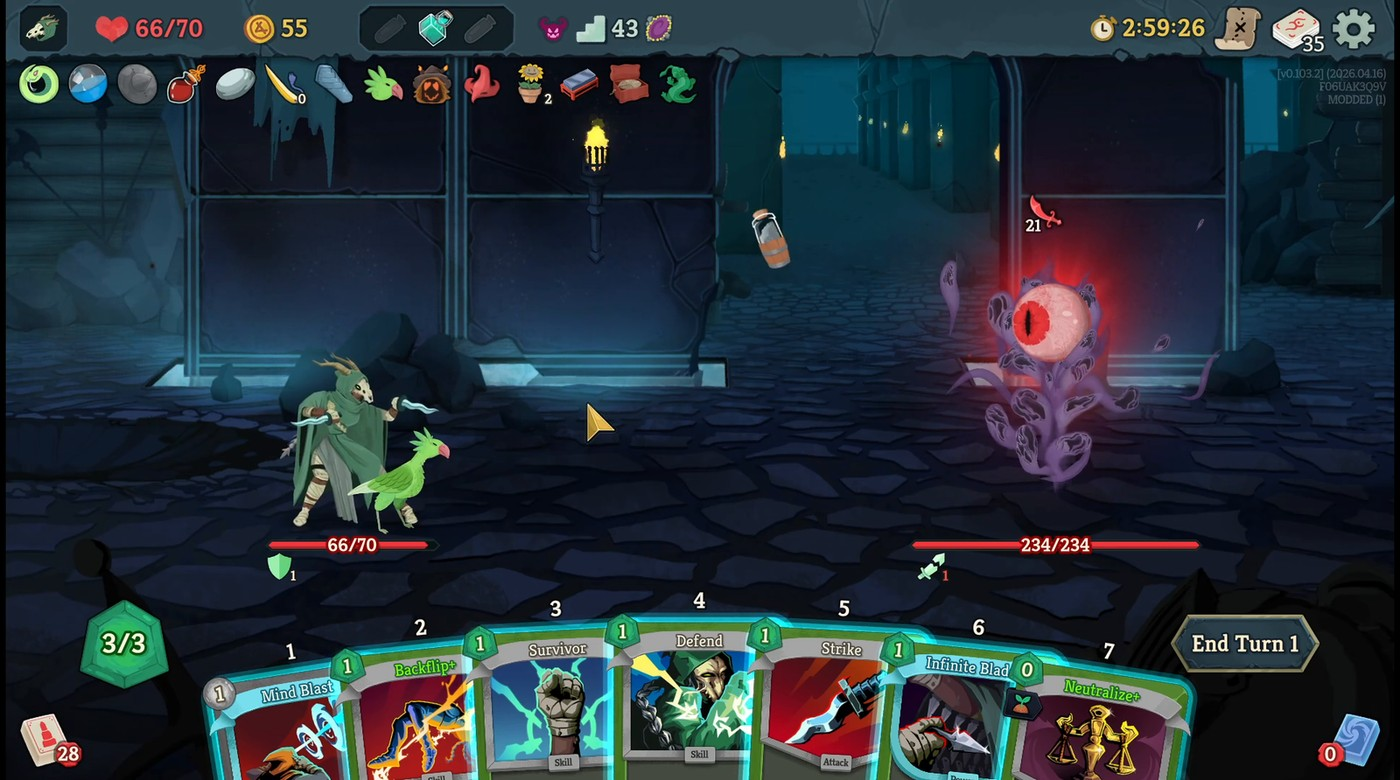
\includegraphics[width=.48\textwidth]{figures/workflow/sts2_prompt_exhibit_combat_state.jpg}\hfill
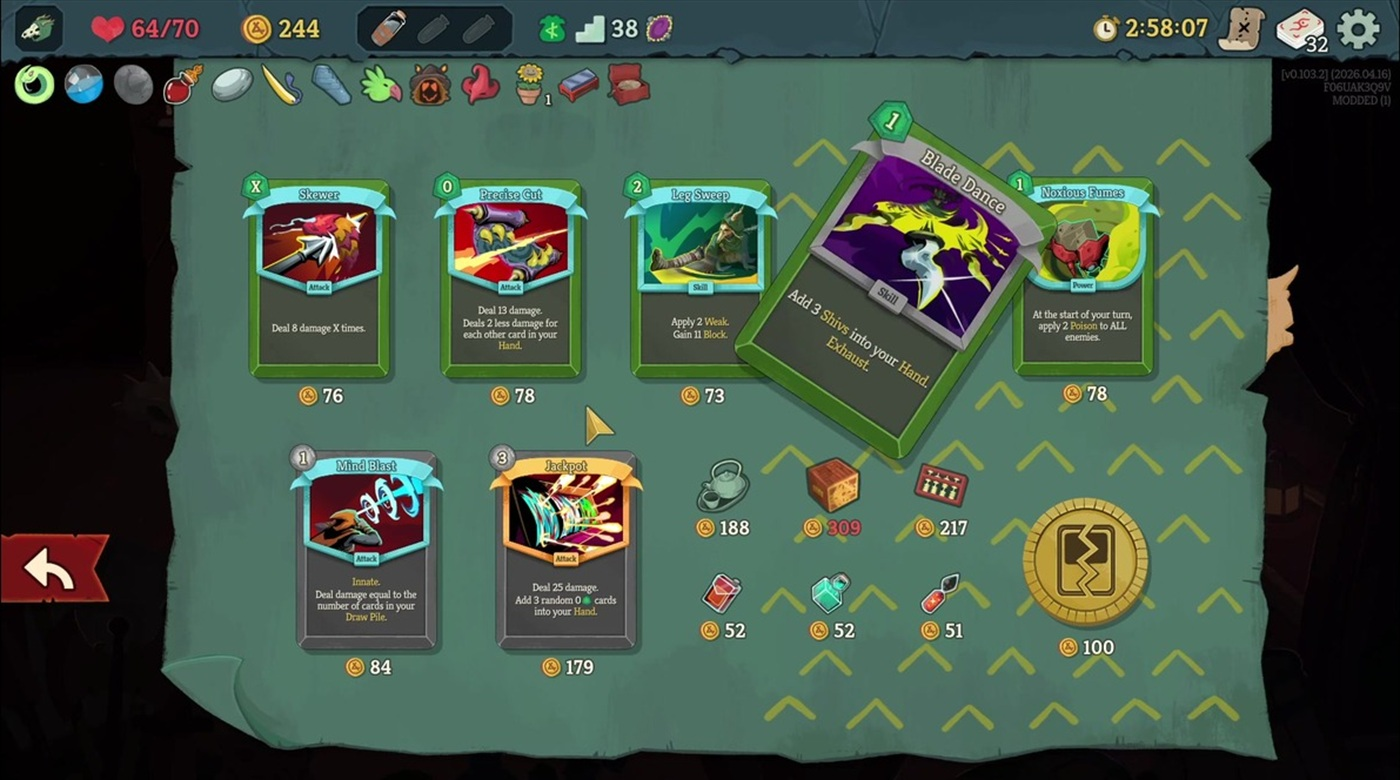
\includegraphics[width=.48\textwidth]{figures/workflow/sts2_prompt_exhibit_shop_state_1400x780.jpg}
\caption{Decision states used in the prompt exhibits: combat planning (left) and shop planning (right).}
\label{fig:prompt-exhibit-states}
\end{figure*}

\subsection{Combat decision}
\label{app:full-prompt-combat}

The combat exhibit is the longest example: it includes the shared
system instruction, setup context, retrieved skills, episodic notes,
game rules, and the current round state.

\paragraph{System prompt.}
\LoneFile{Role}{appendix_prompts/combat_system_01_L1_preamble.txt}
\LoneFile{Output schema}{appendix_prompts/combat_system_02_L1_output_format.txt}
\LthreeFile{Combat rules}{appendix_prompts/combat_system_03_L3_core_combat_rules.txt}
\LfiveFile{HP policy}{appendix_prompts/combat_system_04_L5_hp_conservation.txt}

\paragraph{User prompt: setup and retrieved context.}
\LtwoFile{Combat start}{appendix_prompts/combat_user_setup_01_L2_combat_start.txt}
\LtwoFile{Deck}{appendix_prompts/combat_user_setup_02_L2_current_deck_35_cards.txt}
\LtwoFile{Relics}{appendix_prompts/combat_user_setup_03_L2_relics_14.txt}
\LfourFile{Strategic thread}{appendix_prompts/combat_user_setup_04_L4_strategic_thread.txt}
\LfiveFile{Retrieved skills}{appendix_prompts/combat_user_setup_05_L5_expert_knowledge_retrieved_skills.txt}
\LfourFile{Past experience}{appendix_prompts/combat_user_setup_06_L4_past_experience.txt}
\LfourFile{Past experience}{appendix_prompts/combat_user_setup_07_L4_past_experience.txt}
\LfourFile{Combat guide}{appendix_prompts/combat_user_setup_08_L4_combat_guide.txt}
\LtwoFile{Enemy patterns}{appendix_prompts/combat_user_setup_09_L2_enemy_patterns.txt}
\LfiveFile{Potion strategy}{appendix_prompts/combat_user_setup_10_L5_potion_strategy.txt}
\LfourFile{Card notes}{appendix_prompts/combat_user_setup_11_L4_card_notes_from_experience.txt}
\LthreeFile{Rules}{appendix_prompts/combat_user_setup_12_L3_combat_rules.txt}

\paragraph{User prompt: current combat state.}
\LtwoFile{Round state}{appendix_prompts/combat_user_state_01_L2_round_1_state.txt}
\LtwoFile{Enemies}{appendix_prompts/combat_user_state_02_L2_enemies.txt}
\LtwoFile{Relic counters}{appendix_prompts/combat_user_state_03_L2_relic_counters.txt}
\LtwoFile{Potions}{appendix_prompts/combat_user_state_04_L2_usable_potions.txt}
\LtwoFile{Piles}{appendix_prompts/combat_user_state_05_L2_piles.txt}
\LthreeFile{Active effects}{appendix_prompts/combat_user_state_06_L3_key_effects_active_this_combat.txt}
\LtwoFile{Hand}{appendix_prompts/combat_user_state_07_L2_hand_7_playable_7_total.txt}

\paragraph{Structured response.}
The model returned a structured combat plan: use Powdered Demise,
play Neutralize+, Mind Blast, Backflip+, Infinite Blades, Survivor,
and then end the turn.

\subsection{Shop-planning decision}
\label{app:full-prompt-shop}

The shop exhibit shows the same interface outside combat. To avoid
printing the shared role and generic JSON schema twice, it includes
only the shop-specific system additions and the shop user prompt.

\paragraph{Shop-specific system prompt.}
\LfiveFile{Deck philosophy}{appendix_prompts/shop_system_03_L5_card_deck_philosophy.txt}
\LfiveFile{Two-phase framework}{appendix_prompts/shop_system_04_L5_strategic_deckbuilding_the_two_phase_framework.txt}
\LfiveFile{Phase 1}{appendix_prompts/shop_system_05_L5_phase_1_foundation_no_engine_yet.txt}
\LfiveFile{Phase 2}{appendix_prompts/shop_system_06_L5_phase_2_commitment_engine_acquired.txt}
\LoneFile{Note schema}{appendix_prompts/shop_system_07_L1_output_strategic_note.txt}

\paragraph{User prompt.}
\LfiveFile{Retrieved skills}{appendix_prompts/shop_user_01_L5_expert_knowledge_retrieved_skills.txt}
\LfourFile{Deck insights}{appendix_prompts/shop_user_02_L4_deck_building_insights.txt}
\LfourFile{Card insights}{appendix_prompts/shop_user_03_L4_card_specific_insights.txt}
\LthreeFile{Game knowledge}{appendix_prompts/shop_user_04_L3_game_knowledge.txt}
\LthreeFile{Card mechanics}{appendix_prompts/shop_user_05_L3_card_mechanics_from_game_data.txt}
\LtwoFile{Shop state}{appendix_prompts/shop_user_06_L2_shop.txt}
\LtwoFile{Deck}{appendix_prompts/shop_user_07_L2_current_deck_32_cards.txt}
\LtwoFile{Relics}{appendix_prompts/shop_user_08_L2_relics_ring_of_the_snake_at_the_start_of_each_combat_draw_2_additional_cards_lar.txt}
\LfourFile{Relic synergies}{appendix_prompts/shop_user_09_L4_relic_synergies.txt}
\LfourFile{Gold budget}{appendix_prompts/shop_user_10_L4_gold_budget_analysis.txt}
\LfiveFile{Shop guide}{appendix_prompts/shop_user_11_L5_guide.txt}
\LfourFile{Card notes}{appendix_prompts/shop_user_12_L4_card_notes.txt}
\LoneFile{Task}{appendix_prompts/shop_user_13_L1_your_task.txt}
\LthreeFile{Keywords}{appendix_prompts/shop_user_14_L3_keyword_glossary.txt}
\LtwoFile{Items}{appendix_prompts/shop_user_15_L2_items_for_sale.txt}
\LoneFile{Shop-plan schema}{appendix_prompts/shop_user_16_L1_decision_format_shop_plan.txt}

\paragraph{Structured response.}
The model returned a shop plan that buys Blade Dance, Leg Sweep, Mind
Blast, and Swift Potion, while skipping the remaining affordable items
with item-level reasons.
